\chapter{\textit{Introduction}}
\section{Previous Requirements}
the minimum requirements to run properly the application are:
\begin{itemize} \itemsep0pt \parskip0pt \parsep0pt
	\renewcommand{\labelitemi}{$\rightarrow$}
	\item Operative System: Mac OS X, Windows (XP or newer), Linux, Solaris. 32 or 64 bits architectures.
	\item Software: Java 8 (mandatory requirement).
	\item CPU: AMD or Intel {$>$} 1Ghz.
	\item Memory: At least 512Mb availables.
	\item Graphics Card: AMD/ATI Radeon 9500, NVIDIA GeForce 5 FX, Intel GMA 4500, or better.
	\item Screen: minimun resolution 1024x768
\end{itemize}
\newpage

\section{Application Run}
To run the application it's necessary have installed at least the version 8 of the \textit{Java Virtual Machine} (\emph{http://www.java.com/en/download/}).\\
According to the Operative System installed, can run the application directly from the file explorer or through the system console writing:\\ \emph{java -jar jtlc.jar} over the application folder.
When the application start a new file (\textit{jtlc.settings.props}) is created to store the current settings.
In picture \ref{fig:inicial} is detailed  the application main window.

\begin{figure}[H]
	\vspace{0cm}
	\centering
	
\includegraphics[width=385px]{imagenes/main}
	\centering
	\vspace{-0.4cm}
	\caption{Application initial screen.}
	\label{fig:inicial}
	\vspace{-0.25cm}
\end{figure}
\newpage

\section{Application Settings}
The application settings allows to the user change the system language, projects workspace and enable or disable animations (like screen transition between each analysis screen). To access the settings screen go to \emph{Edit} \ding{222} \emph{Change settings} on the main menu bar.
In the settings screen use \emph{Directory Selector} to change current workspace, the language select to change the application languge, move the animations switch to enable or disable animations. To save current settings click on the button Accept or press \emph{Enter} key from your keyboard. to discard the current settings click on the button Cancel or press \emph{Esc} key.

\begin{figure}[H]
	\vspace{0cm}
	\centering
	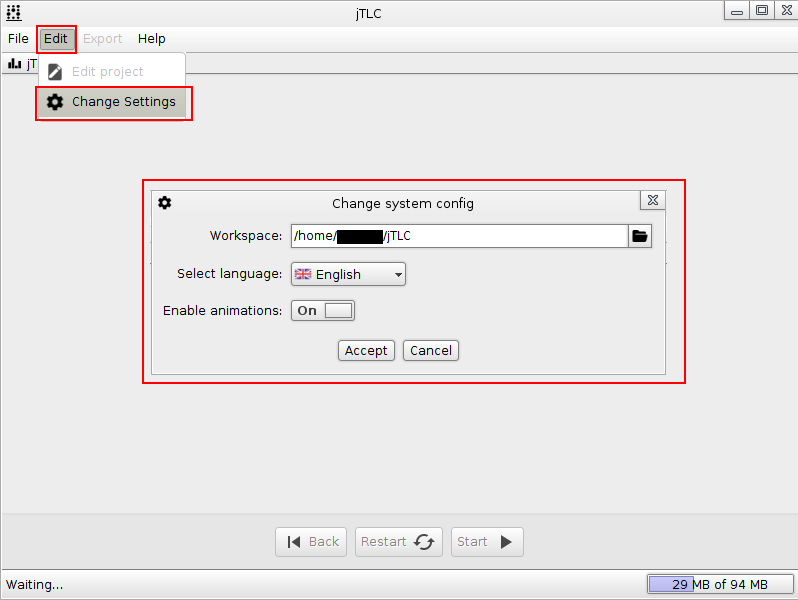
\includegraphics[width=385px]{imagenes/settings}
	\centering
	\vspace{-0.4cm}
	\caption{Application settings.}
	\label{fig:settings}
	\vspace{-0.25cm}
\end{figure}
\newpage

\chapter{\textit{Projects}}
\section*{Start new project}
To start new project...
\begin{figure}[H]
	\vspace{0cm}
	\centering
	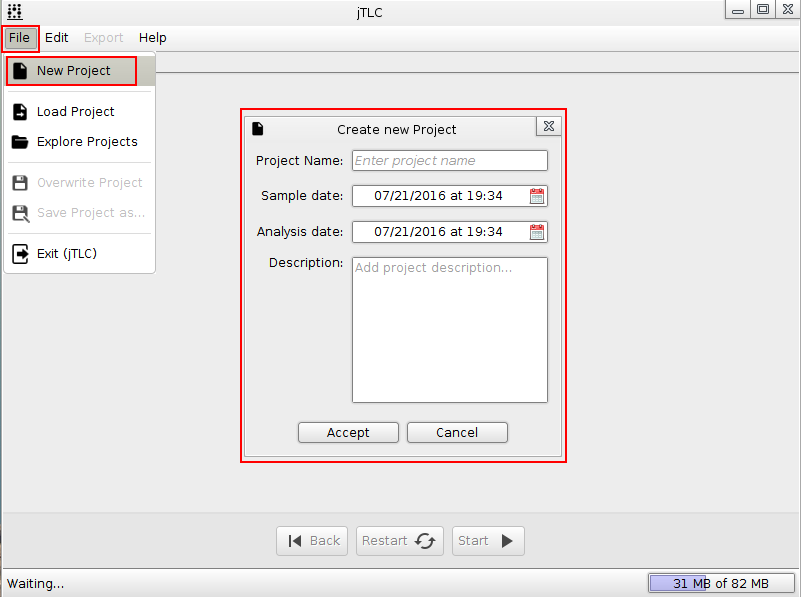
\includegraphics[width=385px]{imagenes/new_project}
	\centering
	\vspace{-0.4cm}
	\caption{New project menu.}
	\label{fig:new_project}
	\vspace{-0.25cm}
\end{figure}
\newpage

\section{Load existent project}
To load a previous project...
\begin{figure}[H]
	\vspace{0cm}
	\centering
	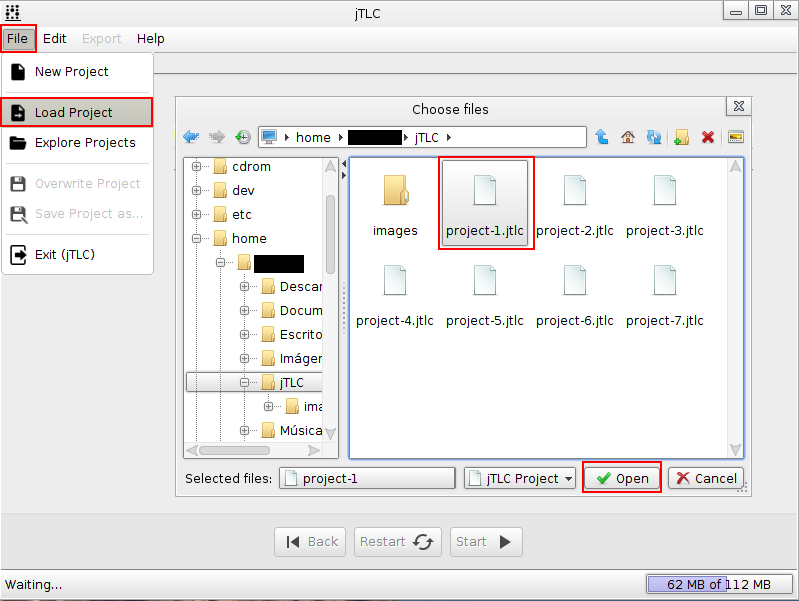
\includegraphics[width=385px]{imagenes/load_project}
	\centering
	\vspace{-0.4cm}
	\caption{New project menu.}
	\label{fig:load_project}
	\vspace{-0.25cm}
\end{figure}
\newpage

\section{Explore projects}
To explore old projects...
\begin{figure}[H]
	\vspace{0cm}
	\centering
	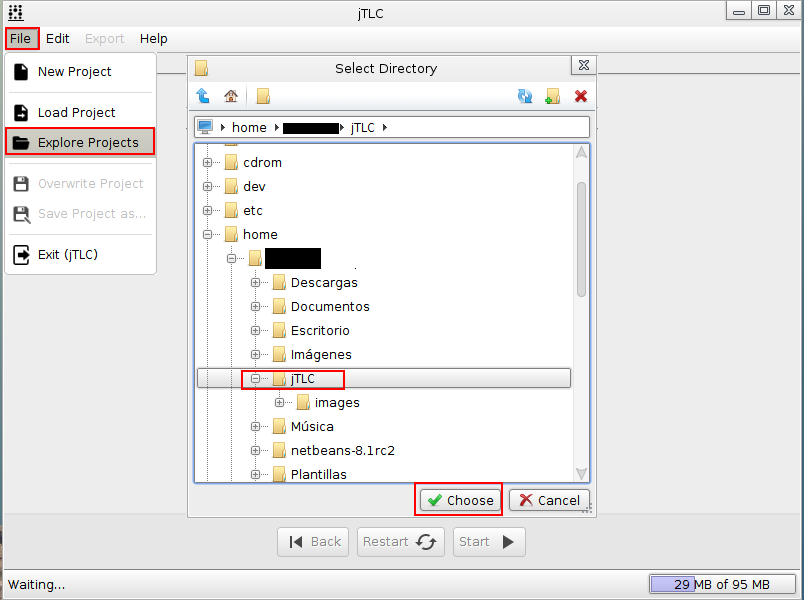
\includegraphics[width=385px]{imagenes/explore_projects}
	\centering
	\vspace{-0.4cm}
	\caption{Explore projects.}
	\label{fig:explore_projects}
	\vspace{-0.25cm}
\end{figure}

\begin{figure}[H]
	\vspace{0cm}
	\centering
	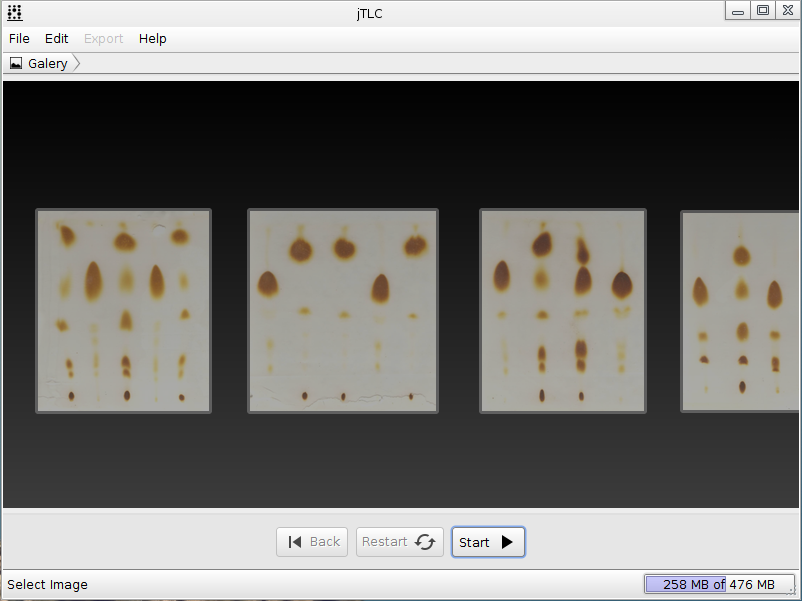
\includegraphics[width=385px]{imagenes/gallery}
	\centering
	\vspace{-0.4cm}
	\caption{Projects gallery.}
	\label{fig:gallery}
	\vspace{-0.25cm}
\end{figure}
\newpage

\section{Edit Project}
To edit a project...
\begin{figure}[H]
	\vspace{0cm}
	\centering
	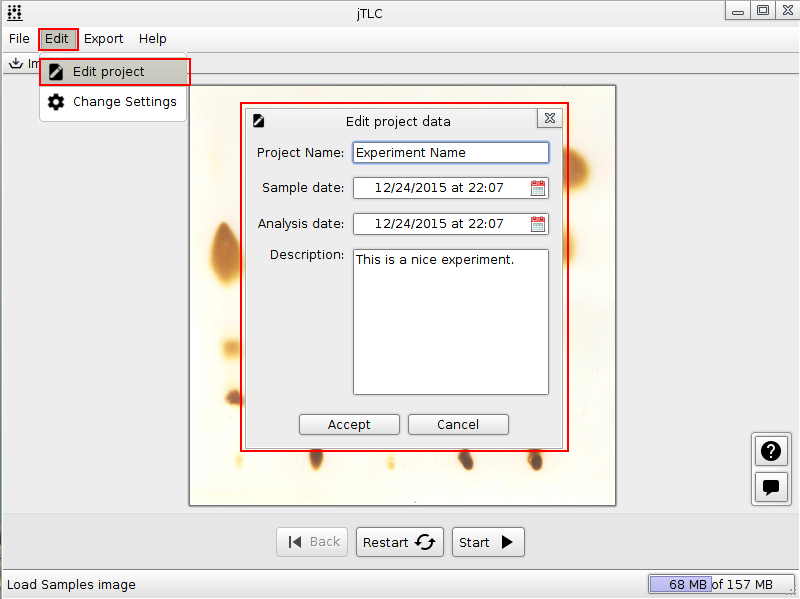
\includegraphics[width=385px]{imagenes/edit_project}
	\centering
	\vspace{-0.4cm}
	\caption{Edit project data.}
	\label{fig:edit_project}
	\vspace{-0.25cm}
\end{figure}

\section{Save Project}
To save current project...

\chapter{Samples Analysis}
\section{Image Load}
\begin{figure}[H]
	\vspace{0cm}
	\centering
	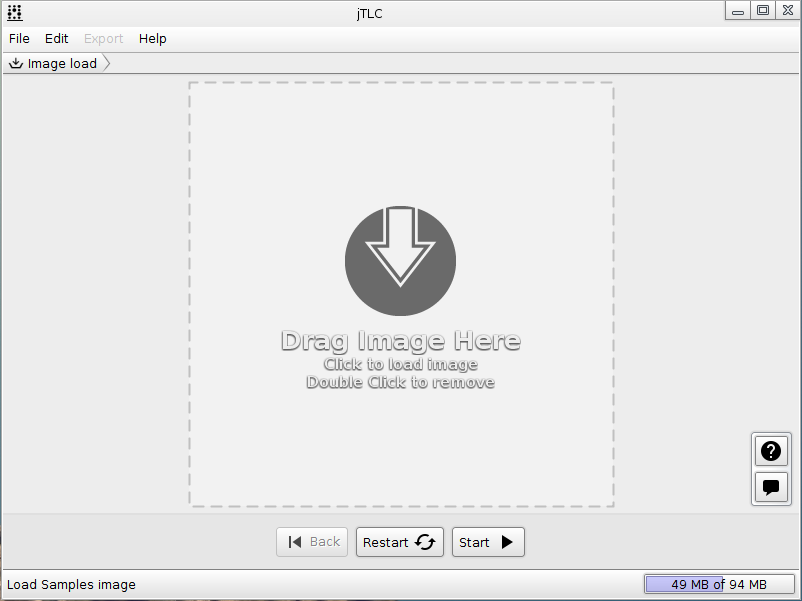
\includegraphics[width=385px]{imagenes/drop}
	\centering
	\vspace{-0.4cm}
	\caption{Load experiment image.}
	\label{fig:image_load}
	\vspace{-0.25cm}
\end{figure}

\section{Image Crop}
\begin{figure}[H]
	\vspace{0cm}
	\centering
	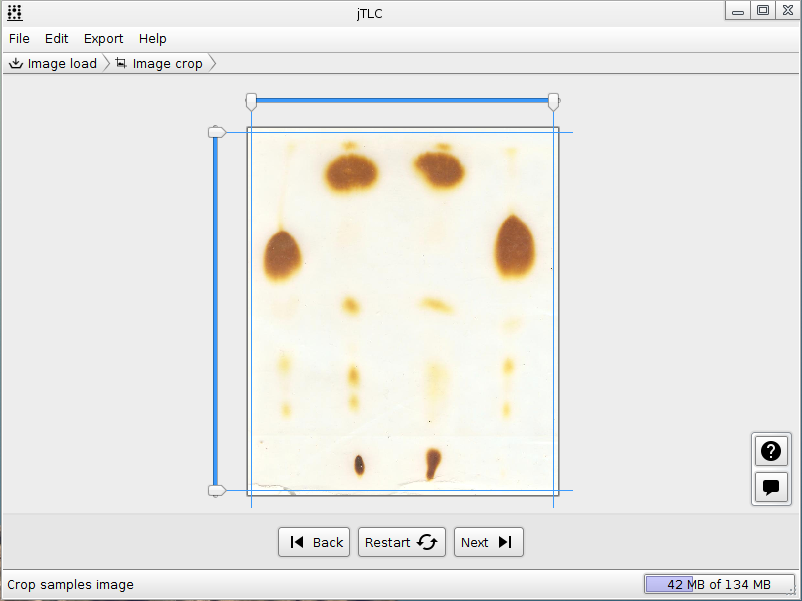
\includegraphics[width=385px]{imagenes/crop}
	\centering
	\vspace{-0.4cm}
	\caption{Crop samples image.}
	\label{fig:image_cut}
	\vspace{-0.25cm}
\end{figure}

\section{Image Rotation}
\begin{figure}[H]
	\vspace{0cm}
	\centering
	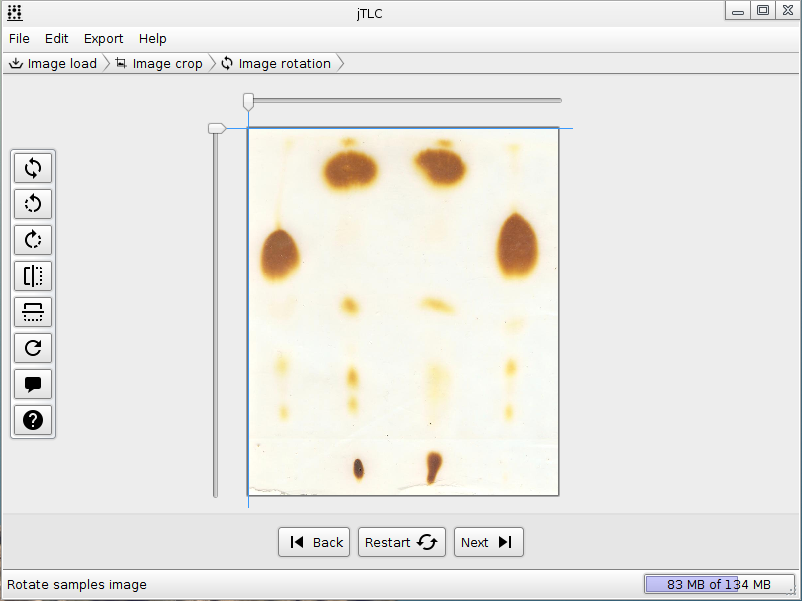
\includegraphics[width=385px]{imagenes/rotate}
	\centering
	\vspace{-0.4cm}
	\caption{Rotate and flip samples image.}
	\label{fig:image_rot}
	\vspace{-0.25cm}
\end{figure}

\section{Samples Selection}
\begin{figure}[H]
	\vspace{0cm}
	\centering
	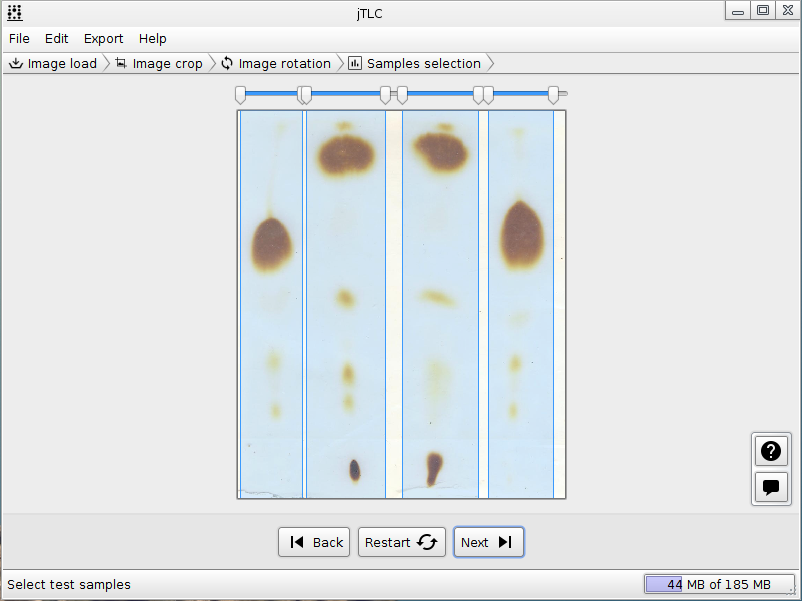
\includegraphics[width=385px]{imagenes/selection}
	\centering
	\vspace{-0.4cm}
	\caption{Individual samples selection.}
	\label{fig:image_samples_selection}
	\vspace{-0.25cm}
\end{figure}

\section{Samples Special Points}
\begin{figure}[H]
	\vspace{0cm}
	\centering
	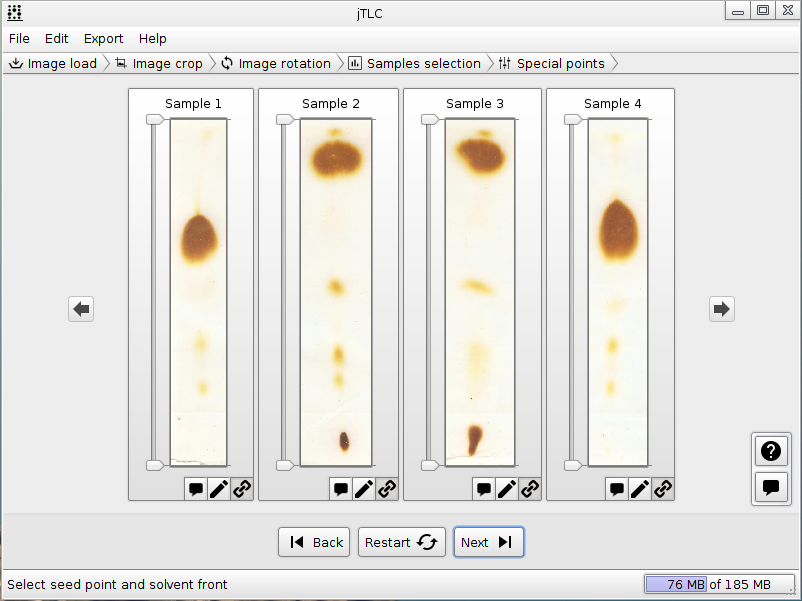
\includegraphics[width=385px]{imagenes/points}
	\centering
	\vspace{-0.4cm}
	\caption{Samples data and special points selection.}
	\label{fig:image_samples_special_points}
	\vspace{-0.25cm}
\end{figure}

\section{Samples Peaks Selection}
\begin{figure}[H]
	\vspace{0cm}
	\centering
	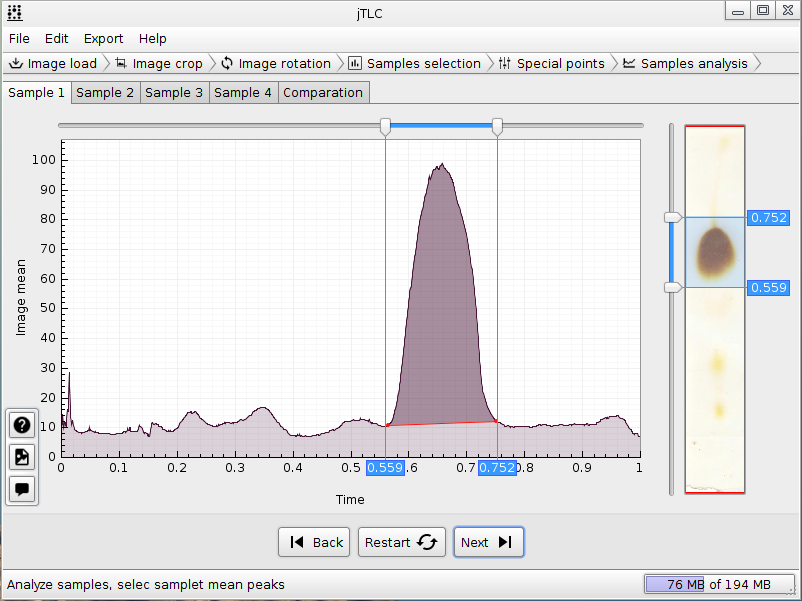
\includegraphics[width=385px]{imagenes/analysis}
	\centering
	\vspace{-0.4cm}
	\caption{Individual samples peaks selection.}
	\label{fig:image_samples_peaks}
	\vspace{-0.25cm}
\end{figure}

\section{Samples Comparation}
\begin{figure}[H]
	\vspace{0cm}
	\centering
	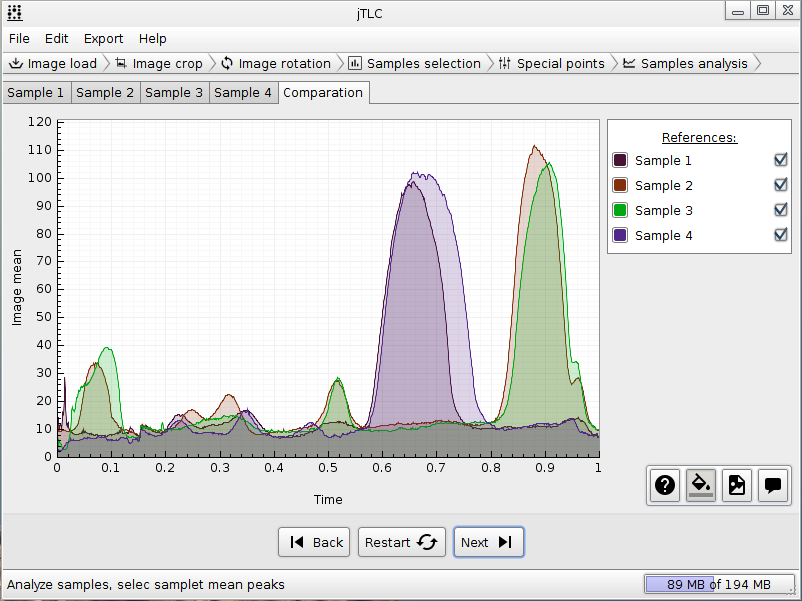
\includegraphics[width=385px]{imagenes/comparation}
	\centering
	\vspace{-0.4cm}
	\caption{Experiment samples mean comparation.}
	\label{fig:image_samples_comparation}
	\vspace{-0.25cm}
\end{figure}

\section{Analysis Results}
\begin{figure}[H]
	\vspace{0cm}
	\centering
	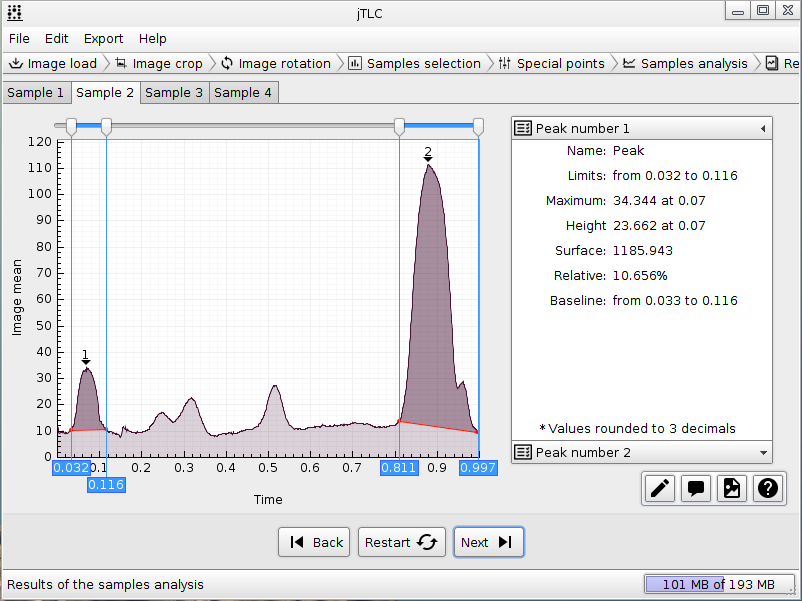
\includegraphics[width=385px]{imagenes/peaks}
	\centering
	\vspace{-0.4cm}
	\caption{Samples peaks analysis results.}
	\label{fig:image_analysis_results}
	\vspace{-0.25cm}
\end{figure}

\section{Analysis Reports}
\begin{figure}[H]
	\vspace{0cm}
	\centering
	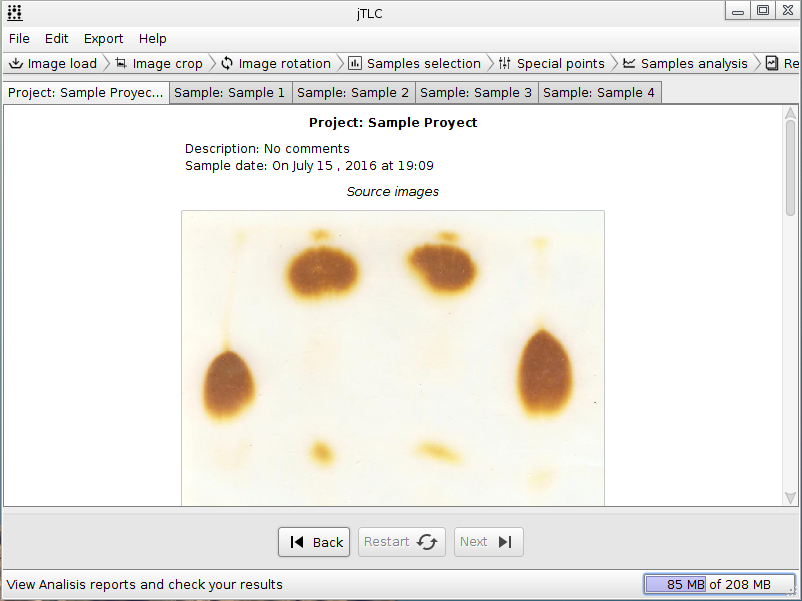
\includegraphics[width=385px]{imagenes/reports}
	\centering
	\vspace{-0.4cm}
	\caption{Samples analysis reports.}
	\label{fig:image_analysis_reports}
	\vspace{-0.25cm}
\end{figure}

\chapter{Data Export}
\section{Export images}
To export project data...

\section{Export reports}
To export project data...

\section{Export data}
\subsection{Export mean}
To export project data...

\subsection{Export plain data}
To export project data...